\documentclass[hidelinks]{article}

\title{Numerical Methods for \\ High Performance Computing}
\author{Lorenzo Schiavone}
\date{\today}
\usepackage{graphicx}
\usepackage{hyperref}
\usepackage[utf8]{inputenc}
\usepackage{amsmath, amssymb, amsthm, mathtools, mathrsfs}
\usepackage[margin=1in]{geometry}

\usepackage[shortlabels]{enumitem}
\usepackage[colorinlistoftodos]{todonotes}
\usepackage{listings}
\usepackage{matlab-prettifier}
\usepackage{color}
\usepackage{subcaption}
\usepackage{caption}
\usepackage{float} 
\usepackage{comment}

\usepackage{graphics}
\usepackage{multicol}

\usepackage{tikz-3dplot}


\theoremstyle{definition}
\newtheorem{ex}{Exercise}

\usepackage{algorithm, algorithmicx}
\usepackage{algpseudocode}

\usepackage{array}
\usepackage{booktabs}

\lstset{
  language=C,
  basicstyle=\ttfamily\small,
  keywordstyle=\color{blue}\bfseries,
  stringstyle=\color{green!60!black},
  commentstyle=\color{gray}\itshape,
}
\DeclareMathOperator{\divg}{div}

\begin{document}
\maketitle
\tableofcontents

\section{Problem Statement and Strong Formulation}
Consider the Transient Convection-Diffusion Equation 

\begin{equation}\tag{$D$}\label{eq:strong}
    \begin{aligned}
    \frac{\partial}{\partial t}u -K \Delta u + \divg(\beta u) &=0 && \text{in } \Omega, \\
    u(\mathbf{x}) &= 1 && \text{for } \mathbf{x} = \mathbf{0}  \\
    \nabla u \cdot \nu &= 0 && \text{for } \mathbf{x}\in \partial\Omega \setminus \{\mathbf{0}\} 
\end{aligned}
\end{equation}
for $\Omega = [0,1] \times [0,1]\times [0,1]$, where $u=u(x,y,z)$ represents the scalar concentration of a solute dissolved in a fluid moving with velocity $\beta$ constant and homogenous and $K=\texttt{diag}(K_1,K_2,K_3)$ is the diffusion matrix assumed constant as well.

\begin{figure}[H]
\begin{center}
\tdplotsetmaincoords{75}{15}
\begin{tikzpicture}[tdplot_main_coords, scale=2]

% Draw cube edges
\draw[thick] (0,0,0) -- (1,0,0);  % x-axis edge
\draw[thick] (0,0,0) -- (0,1,0);  % y-axis edge
\draw[thick] (0,0,0) -- (0,0,1);  % z-axis edge

\draw[thick] (1,0,0) -- (1,1,0);
\draw[thick] (1,0,0) -- (1,0,1);

\draw[thick] (0,1,0) -- (1,1,0);
\draw[thick] (0,1,0) -- (0,1,1);

\draw[thick] (0,0,1) -- (1,0,1);
\draw[thick] (0,0,1) -- (0,1,1);

\draw[thick] (1,1,0) -- (1,1,1);
\draw[thick] (1,0,1) -- (1,1,1);
\draw[thick] (0,1,1) -- (1,1,1);

% Red dot at origin
\filldraw[red] (0,0,0) circle (1pt);         

\node[black] at (0.5, 0.5, 0.5) {$\Omega$};

\end{tikzpicture}
\end{center}
\caption{Domain of study.}
\end{figure}

\section{Weak Galerkin Formulation}
The Weak Formulation of (\ref{eq:strong}) is: find $u \in H^1(\Omega)$ such that boundary conditions hold and 

\begin{equation}\tag{$W$}\label{eq:weak}
\int_\Omega \frac{\partial u}{\partial t } v \,d\Omega + \int_\Omega K \nabla u \cdot \nabla v \,d\Omega + \int_\Omega \divg( \beta u) v\,d\Omega = 0
\end{equation}

for every $v \in H^1_0(\Omega)$, where we have integrated by part the first term and the boundary term vanishes because $v \in H^1_0(\Omega)$.

Now, considering the discretization $\mathcal{T}_h$ of $\Omega$ with nodes $\mathcal{N}_h = \{\mathbf{x}_1, \dots, \mathbf{x}_{n_\text{nodes}}\}$ and tetrahedral finite elements $\mathcal{E}_h$, we can approximate the function space $H^1(\Omega)$ with 
\[
\mathcal{V}_h = \text{span}\, \{\phi_1, \dots, \phi_{n_\text{nodes}} \}, 
\]
where the $\phi_i$ are the piecewise linear Lagrangian basis function. Then, we can write the approximate solution $u_h(t) = \sum_{j=0}^{n_\text{nodes}} u_j(t) \phi_j$ and, as $\mathcal{V}_h$ is a finite dimensional vector space, is enough to verify Equation (\ref{eq:weak}) for the basis functions $\phi_i$. It yields the Weak Galerkin Formulation: find $u_h(t) \in \mathcal{V}_h$ such that boundary conditions hold and

\begin{equation}\tag{$W_h$}\label{eq:weakGalerkin1}
\int_\Omega \sum_{j=1}^{n_\text{nodes}} u'_j(t)\phi_j\phi_i \,d\Omega +\int_\Omega \sum_{j=1}^{n_\text{nodes}} u_j(t) K \nabla \phi_j \cdot \nabla \phi_i \,d\Omega + \int_\Omega \sum_{j=1}^{n_\text{nodes}} u_j(t) \divg( \beta \phi_j) \phi_i\,d\Omega = 0
\end{equation}

or 

\begin{equation}\tag{$W_h$}\label{eq:weakGalerkin2}
\sum_{j=1}^{n_\text{nodes}} u'_j(t) \left( \int_\Omega \phi_j\phi_i \,d\Omega \right) + \sum_{j=1}^{n_\text{nodes}} u_j(t) \left(\int_\Omega K  \nabla \phi_j \cdot \nabla \phi_i \,d\Omega\right) + \sum_{j=1}^{n_\text{nodes}} u_j(t) \left(\int_\Omega  \divg( \beta \phi_j) \phi_i\,d\Omega\right) = 0
\end{equation}

that in matrix form reads \[ P\mathbf{u}' + H\mathbf{u} + B\mathbf{u} = 0\] where $\mathbf{u} = (u_1, \dots, u_{n_\text{nodes}})^T$, and the mass matrix $P$, the diffusion stiffness matrix $H$ and the non-symmetric convective matrix $B$ have components, respectively,
\[P_{ij} = \int_\Omega \phi_j \phi_i\, d\Omega ,\quad\quad H_{ij} = \int_\Omega K \nabla \phi_j \cdot \nabla \phi_i\, d\Omega \quad \text{and} \quad B_{ij} = \int_\Omega  \divg( \beta \phi_j) \phi_i\,d\Omega.\]

\section{Finite Elements and Assembly}

Inside each tetrahedral element $e\in\mathcal{E}$ with vertices $\mathbf{x}_i, \mathbf{x}_j, \mathbf{x}_k, \mathbf{x}_m$ only the corresponding basis function $\phi_i,\phi_j,\phi_k,\phi_m$ are non zero. Their local expression is 
\[
\phi_l^{(e)} (x,y,z)= \frac{a_l + b_l x + c_l y + d_l z}{6V^{(e)}} \quad \text{for } l \in \{i,j,k,m\},
\]
where $V^{(e)}$ is the surface measure of the element,
\[
V^{(e)} = \frac{1}{6}\det \left(\begin{bmatrix}
    1 & x_i & y_i & z_i \\ 1 & x_j & y_j & z_j\\ 1 & x_k & y_k & z_k \\ 1 & x_m & y_m & z_m
\end{bmatrix} \right),
\]
and the coefficients $\mathbf{a}, \mathbf{b}, \mathbf{c}, \mathbf{d}$ are computed so that $\phi_l(\mathbf{x_r}) = \delta_{lr}$, i.e., 

\begin{align*}
a_i &= & b_i &= & c_i &= & d_i &= \\
a_j &= & b_j &= & c_j &= & d_j &= \\
a_k &= & b_k &= & c_k &= & d_k &= \\
a_m &= & b_m &= & c_m &= & d_m &= 
\end{align*}
Then, \[\nabla \phi_i^{(e)} = \frac{1}{2\Delta^{(e)}}\begin{bmatrix}
    b_i \\ c_i
\end{bmatrix} \] is constant and the local diffusion stiffness matrix is 
\[ H_{ij}^{(e)} = K \int_e \frac{1}{2\Delta^{(e)}}(b_i, c_i)^T \cdot \frac{1}{2\Delta^{(e)}}(b_j, c_j)^T \,d\Omega = K \frac{\Delta^{(e)}}{{4\Delta^{(e)}}^2} (b_ib_j + c_ic_j) = \frac{K}{4\Delta^{(e)}} (b_ib_j + c_ic_j). \]
Compactly, if we collect $\mathbf{b} = \begin{bmatrix} b_i & b_j & b_k \end{bmatrix}$ and, likewise $\mathbf{c} = \begin{bmatrix} c_i & c_j & c_k \end{bmatrix}$, we can write 
\[ H^{(e)} = \frac{K}{4\Delta^{(e)}}(\mathbf{b}^T\mathbf{b} + \mathbf{c}^T\mathbf{c}).
\]
\paragraph{Convective Matrix}
Moreover, since \[
\divg (\beta \phi_j) = \partial_x (\beta_x \phi_j) + \partial_y (\beta_y \phi_j) = \beta_x \partial_x \phi_j +  \beta_y \partial_y \phi_j = \beta \cdot \nabla \phi_j = \frac{1}{2\Delta^{(e)}}\left(\beta \cdot \begin{bmatrix}
    \mathbf{b} \\
    \mathbf{c}
\end{bmatrix} \right)_j =: \frac{1}{2\Delta^{(e)}} \sigma_j,
\] 
where $\sigma$ is the row vector $\beta \cdot \begin{bmatrix}
    \mathbf{b} \\
    \mathbf{c}
\end{bmatrix}$ for brevity, and
\[
\int_e \phi_i \, d\Omega = \frac{1}{3} \Delta^{(e)} \quad \text{as} \quad \phi^{(e)}_i + \phi^{(e)}_j + \phi^{(e)}_k = 1,
\]
we have that the local convective matrix is
\[
B_{ij}^{(e)} = \int_e \divg (\beta \phi_j) \phi_i \, d\Omega = \frac{1}{2\Delta^{(e)}}\sigma_j \int_e \phi_i \, d\Omega = \frac{1}{2\Delta^{(e)}}\sigma_j \frac{1}{3} \Delta^{(e)} = \frac{1}{6} \sigma_j.
\]
In matrix form,
\[
B^{(e)} = \frac{1}{6} \begin{bmatrix} \sigma \\ \sigma \\ \sigma
\end{bmatrix},
\]
where the rows are equal as the coefficients are independent of the row index.

\paragraph{Stabilization Matrix} The streamline upwind diffusion matrix in the element $e\in\mathcal{E}$ is given by
\[
S_{ij}^{(e)} = \tau \int_e \frac{h^{(e)}}{K^{(e)}|\beta^{(e)}|}(\beta^{(e)}\cdot \nabla \phi_i)(\beta^{(e)}\cdot \nabla \phi_j)\, d\Omega,
\]
where $\tau$ is an hyperparameter to tune how much numerical diffusion to add for stabililization, $h^{(e)}$ is the diameter of the element, $K^{(e)} = \|K_{|e}\|_\infty$ and $\beta^{(e)}$ is the elemental velocity vector.
As $\beta$ and $K$ are constant by assumption and $h^{(e)}=h$, equal for any element, as the triangulation is regular, the coefficients could be computed as 
\[
S_{ij}^{(e)} = \tau \frac{h}{K|\beta|}\int_e (\beta^{(e)}\cdot \nabla \phi_i)(\beta^{(e)}\cdot \nabla \phi_j)\, d\Omega = \tau \frac{h}{K|\beta|} \frac{\sigma_i}{2\Delta^{(e)}} \frac{\sigma_j}{2\Delta^{(e)}} \int_e \,d\Omega = 
\tau \frac{h}{4\Delta^{(e)}K|\beta|}\sigma_i\sigma_j
\] that in matrix form is 
\[
S^{(e)} = \tau \frac{h}{4\Delta^{(e)}K|\beta|} \sigma^T \sigma.
\]

\section{Imposing Boundary Conditions}
Instead of imposing Dirichlet boundary condition with the penalty term method, we follow an exact standard general preocedure.
As the basis functions are chosen to be \emph{Lagrangian}, i.e., there is a basis function $\phi_i$ for each node $N_i$ and $\phi_i(N_j)=\delta_{ij}$, for $u(x) = \sum_i u_i\phi_i(x)$ the coefficient $u_i$ directly represents the value of $u(x)$ evaluated at node $N_i$.

Dirichlet Boundary Conditions on node $N_{\bar{i}}$ are enforced by fixing the corresponding unknown, e.g. $u_{\bar{i}}=\overline{u}$. Since then $u_{\bar{i}}$ is not an unknown anymore, the system can be simplified by replacing its corresponding row with $u_{\bar{i}}=\overline{u}$ and updating other rows by moving terms involving $u_{\bar{i}}$ to the right hand side. For instance, the $i$-th row
\[ \sum_{j=1}^{N_h}a_{ij}u_j = f_i\]
becomes
\[ \sum_{j\neq \bar{i}}a_{ij}u_j = f_i - \overline{u}a_{i\bar{i}}. \]

The implementation follows this approach. First, we store the columns of the matrix corresponding to the nodes with Dirichlet Boundary conditions. Then, we set to zero the corresponding rows and columns, and set to one the diagonal entries, as in the following code snippet, where in the node of index \texttt{dirnodes} we impose the value \texttt{dirval}:
\begin{lstlisting}[style=Matlab-editor]
    A4update = A(:,dirnodes); % store the columns for Dirichlet bc
    nBound = length(dirnodes);
    A(dirnodes, :) = sparse(nBound, size(H,2)); %zero out solved rows
    A(:, dirnodes) = sparse(size(H,1), nBound); %zero out columns
    A(dirnodes(:,1),dirnodes(:,1)) = speye(nBound); %one in the diagonal 
\end{lstlisting}
Finally, with the right hand side $\mathbf{f}$ and the boundary conditions \texttt{bound}, we enforce them with
\begin{lstlisting}[style=Matlab-editor]
    q = f - A4update * dirval; 
    q(dirnodes) = dirval; 
\end{lstlisting}
and the final linear system is \[ A u = q.\]

\section{Numerical Solution}
We solve numerically the equation in study for $K = [0.001, 0.01, 0.1, 1]$. The mesh provided is a structural mesh made of isosceles rectangular triangle with $l=1/20$ and hypotenusa $h= \sqrt{2}/20$. With $\beta = \begin{bmatrix}
    1 & 3
\end{bmatrix}^T $ oscillations occurr starting from $K = 0.01$ when convection dominates diffusion. The ``pseudo" Peclet number for the mesh is computed as $\mathbb{P}\!e =|\beta| h / K$ and the values are summarized in Table \ref{tab:peclet}.

\begin{table}[H]
    \centering
    \begin{tabular}{c|c}
        K & $\mathbb{P}\!e$ \\
        \hline
        1 & 0.2236 \\
        0.1 & 2.236 \\
        0.01 & 22.36 \\
        0.001 & 223.6
    \end{tabular}
    \caption{Pseudo Peclet number for different values of $K$ for the considered mesh and $\beta = \begin{bmatrix}
    1 & 3
\end{bmatrix}^T$.}\label{tab:peclet}
\end{table}
We can clearly notice that for $K = 1$, the Peclet number is well inside the stable region $\mathbb{P}\!e \lesssim 2$, whereas for $K = 0.1$, the Peclet number lies in a transitional or uncertain zone $2 \lesssim \mathbb{P}\!e \lesssim 3$.
Viceversa for $K\leq 0.01$ the Peclet number is in the unstable region. 

Numerical simulation without stabililization term confirm these results. Figure \ref{fig:nostab1} and \ref{fig:nostab} show the obtained solution for different values of $K$. Oscillations are evident for $K\leq 0.01$. As $u$ represents a concentration normalized between 0 and 1, the solutions with $K\leq 0.01$ are non physical because they have oscillations with negative values and values greater than one.

\begin{figure}[H]\centering
    
    \begin{subfigure}[t]{0.45\textwidth}
        \centering
        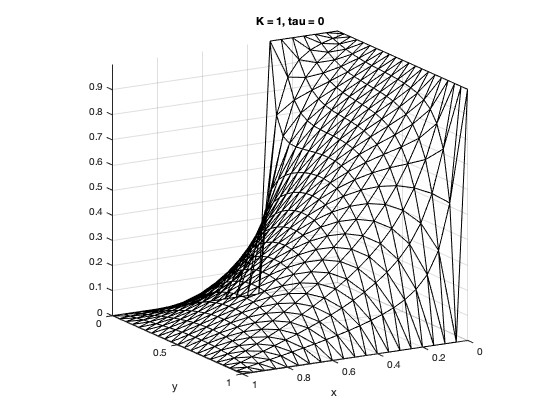
\includegraphics[width=\textwidth]{pic/k1t0.jpg}
    \end{subfigure}
    \hfill
    \begin{subfigure}[t]{0.45\textwidth}
        \centering
        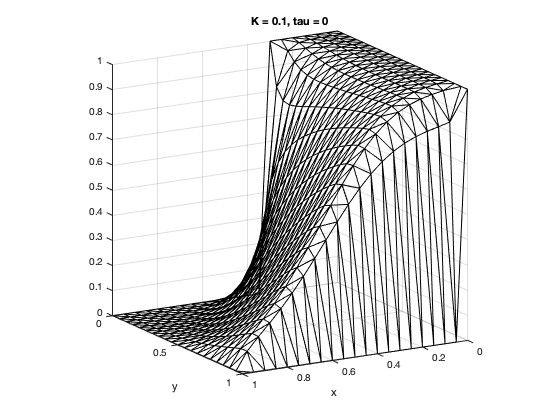
\includegraphics[width=\textwidth]{pic/k01t0.jpg}
    \end{subfigure}
    \caption{Numerical solution of the Convection-diffusion equation with linear Galerkin elements without stabililization for $K=1$ on the left and $K=0.1$ on the right.}\label{fig:nostab1}

\end{figure}
\begin{figure}[H]\centering
    
    \begin{subfigure}[t]{0.45\textwidth}
        \centering
        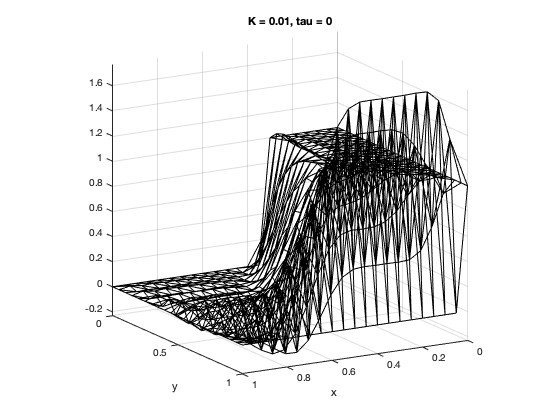
\includegraphics[width=\textwidth]{pic/k001t0.jpg}
    \end{subfigure}
    \hfill
    \begin{subfigure}[t]{0.45\textwidth}
        \centering
        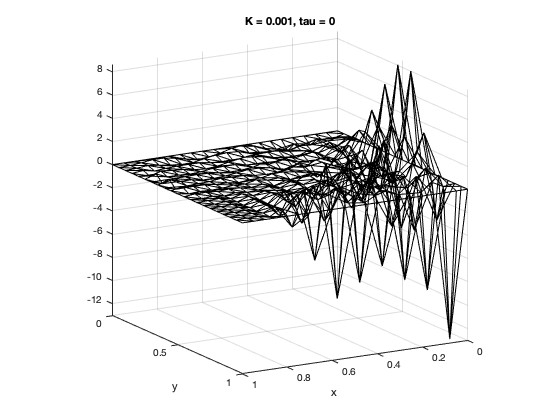
\includegraphics[width=\textwidth]{pic/k0001t0.jpg}
    \end{subfigure}

    \caption{Numerical solution of the Convection-diffusion equation with linear Galerkin elements without stabililization for $K=0.01$ on the left and $K=0.001$ on the right.}
    \label{fig:nostab}
\end{figure}

\section{Stabilized Solution}
For $K=0.01$ and $K=0.001$ we have to find the smallest amount of numerical stabililization diffusion to stabilize the solution of the stabilized linear system \[
(H + B + S)u = 0 \quad \text{s.t. $u$ satisfies BC.}
\] For $K=0.001$ we choose $\tau = 0.005$ and $\tau = 0.01$ for $K=0.01$. Figure \ref{fig:stab} has the stabilized solution for the corresponding value of $K$.

\begin{figure}[H]
     \begin{subfigure}[t]{0.45\textwidth}
        \centering
        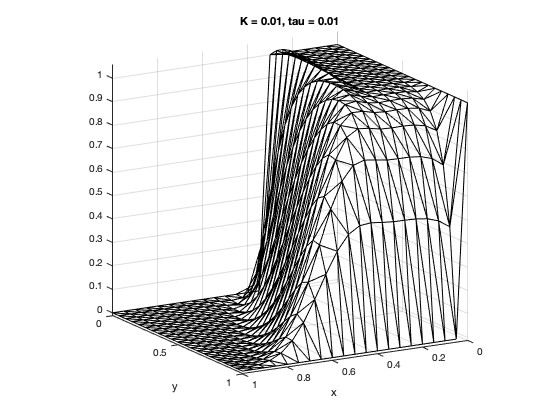
\includegraphics[width=\textwidth]{pic/k001t001.jpg}
    \end{subfigure}
    \hfill
    \begin{subfigure}[t]{0.45\textwidth}
        \centering
        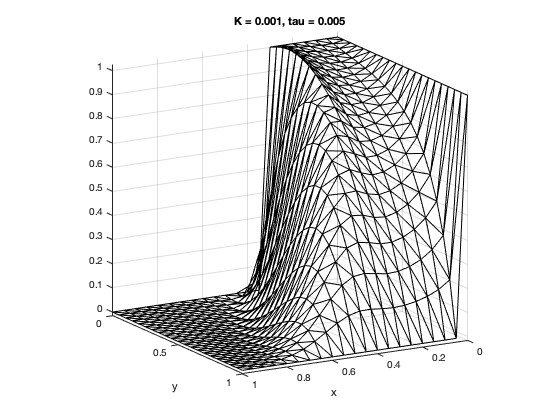
\includegraphics[width=\textwidth]{pic/k0001t0005.jpg}
    \end{subfigure}
    \caption{Stabilized solution for $K=0.01$ and $K=0.001$.}\label{fig:stab}
\end{figure}

\section{Mass Balance}
One can check mass balance to certify the goodness of the numerical solution. Indeed, integrating on $\Omega$ Equation (\ref{eq:strong}), one gets 
\[
-K \int_{\Omega}\divg \nabla u \,d\Omega + \int_{\Omega}\divg(\beta u)\,d\Omega = 0,
\]
that by Green's Lemma is 
\[
0 = - K \int_{\partial\Omega} \nabla u \cdot n \,d\Sigma + \int_{\partial\Omega} u \beta\cdot n \,d\Sigma =: Q_D + Q_C,
\]
where $n$ is the outer normal to $\partial\Omega$ and $d\Sigma$ is the Hausdorff measure on the boundary and we have denoted $Q_D$ and $Q_C$ the diffusive and convective flux respectively.
The convective flux can be computed exactly because the Drichlet boundary conditions fix the value of the solution at the boundary:
\begin{align*}
Q_C &= \int_{\partial\Omega} u \beta\cdot n \,d\Sigma = \int_{\Gamma_1} 1 \cdot (\beta\cdot n) \,d\Sigma + \int_{\Gamma_2} 0 \cdot (\beta\cdot n) \,d\Sigma \\
&= \int_{x=0, y \in [0,1]} (1,3) \cdot (-1,0) \,d\Sigma + \int_{y=0, x \in [0,0.3]} (1,3) \cdot (0,-1) \,d\Sigma = -1 - 3 \cdot 0.3 = -1.9.
\end{align*}
On the other hand, one can compute, denoting $\psi = \sum_{i\in \partial\Omega}\phi_i$,
\begin{align*}
    \sum_{i \in \partial\Omega} (Hu)_i &= \sum_{i\in \partial\Omega} \sum_{j=1}^{n_\text{nodes}} \left(\int_\Omega K \nabla \phi_i \cdot \nabla \phi_j\, d\Omega\right)u_j =  K \int_\Omega \nabla\left(\sum_{i\in \partial\Omega}\phi_i\right) \cdot \nabla \left(\sum_{j=1}^{n_\text{nodes}}u_j\phi_j\right)\, d\Omega \\
    &= \int_\Omega \nabla \psi \cdot \nabla u_h \, d\Omega \overset{(\star)}{\cong} - K \int_\Omega \psi \Delta u_h \, d\Omega + \int_{\partial \Omega} \psi \nabla u_h \cdot n \, d\Sigma = 0 +  K \int_{\partial\Omega} \nabla u \cdot n \,d\Sigma = -Q_D,
\end{align*}
because $\Delta u_h = \sum_j u_j \Delta \phi_j = 0$ almost everywhere as the basis functions are linear and $\psi_{| \partial \Omega} = 1$. On $(\star)$ the equality is up to net flux on edges with a single point on the boundary. 

\paragraph{Numerical results}
The balance of fluxes in the numerical solutions are not satisfied, as one can read in Table \ref{tab:diffflux}. However, we cannot check if the difference between convective and diffusive flux decreases for finer meshes as we are provided only with one.
It is relevant to notice that when stabililization numerical diffusion is added, the diffusion flux decreases as the numerical diffusion flux is predominant.

\begin{table}[H]
    \centering
    \begin{tabular}{c|c|c|c|c|c|c}
  $K$ & 1 & 0.1 & \multicolumn{2}{c|}{0.01} & \multicolumn{2}{c}{0.001} \\
  \hline
  $\tau$    & 0& 0 & 0 & 0.01 & 0 & 0.005 \\
  \hline
  $Q_D$  & 1.619 & 1.085 & 0.2286 & 0.05621 & 0.01191 & -0.001449 \\
\end{tabular}
\caption{Diffusive Flux for different values of $K$ and $\tau$. Convective flux is constant $Q_C=-1.9$.}\label{tab:diffflux}
\end{table}

\end{document}